% Diese Zeile bitte -nicht- aendern.
\documentclass[course=erap]{aspdoc}

%%%%%%%%%%%%%%%%%%%%%%%%%%%%%%%%%
%% TODO: Ersetzen Sie in den folgenden Zeilen die entsprechenden -Texte-
%% mit den richtigen Werten.
\newcommand{\theGroup}{257} % Beispiel: 42
\newcommand{\theNumber}{A205} % Beispiel: A123
\author{Laert Llaveshi \and Till-Ole Lohse \and Yannick Sihler}
\date{Sommersemester 2023} % Beispiel: Wintersemester 2019/20
%%%%%%%%%%%%%%%%%%%%%%%%%%%%%%%%%

% Diese Zeile bitte -nicht- aendern.
\title{Gruppe \theGroup{} -- Abgabe zu Aufgabe \theNumber}

\usepackage{graphicx}%eingefügt, damit wir Grafiken einbauen können.
\usepackage{wrapfig} %eingefügt, damit Text neben Bildern möglich ist.
\usepackage{ragged2e} %eingefügt, damit wir Blocksatz benutzen können unter den Bildern
\usepackage{listings} %eingefügt, damit wir Codeschnippsel einfügen können
\usepackage{cite} %eingefügt, für bibTex Quellen


\begin{document}
\maketitle

\section{Einleitung}

In der vorliegenden Arbeit wird ein Bereich der digitalen Bildverarbeitung (engl. {\textit{Image Processing}}) behandelt, bei dem eine Pixelmanipulation auf einem Bild durchgeführt wird. Ziel ist es dabei, auf einem Bild, welches dem Programm übergeben wird, einen Algorithmus anzuwenden, durch den eine neue Bilddatei erzeugt wird. Hierbei wird ein freiwählbarer Bereich des Bildes ausgeschnitten und im Anschluss mit einem Skalierfaktor vergrössert wie im folgenden Beispiel zu sehen. 

\graphicspath{{images/}}

\begin{figure}[h]
    \centering
    \begin{minipage}[b]{0.4\textwidth}
        \centering
        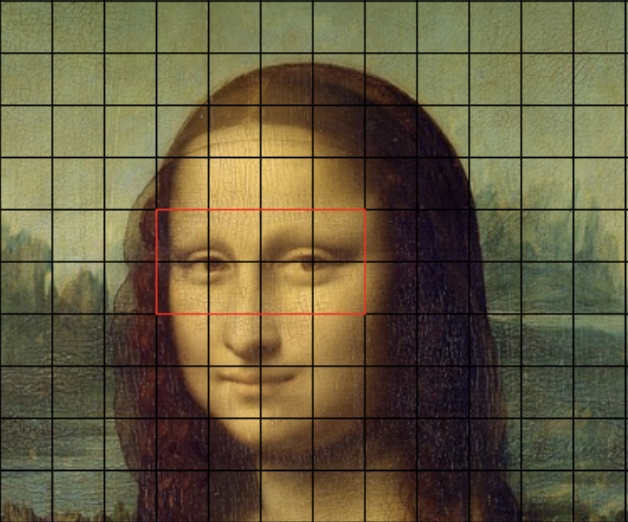
\includegraphics[width=\textwidth]{Monalisa.png}
    \end{minipage}
    \hfill
    \begin{minipage}[b]{0.4\textwidth}
        \centering
        
\includegraphics[width=\textwidth]{mona_lisa_eyes.png}
    \end{minipage}
\end{figure}

Der Fokus liegt im Weiteren auf Bildern mit BMP24-Format. Der Begriff {\textit{BMP}} steht als Abkürzung für {\textit{Bitmap}}.
Eine Bitmap ist ein Array von Bits, die die Farbe jedes Pixels in einem rechteckigen Array von Pixeln angeben.\cite{q2} 

Das BMP24-Format ist ein gängiges Dateiformat, welches für die Speicherung von Bildern benutzt wird. Hierbei liegen Daten in einer unkomprimierten Bitmap im Speicher und jeder Pixel wird durch 24 Bit repräsentiert. Jeder 24 Bit-Block setzt sich zusammen aus jeweils 256 möglichen Farbwerten für die Grundfarben Rot, Blau und Grün. Ein Pixel kann dementsprechend \begin{math}2^{24} = 16.777.216 \end{math} mögliche Farbwerte annehmen. Aufgrund der breiten Farbauswahl für jeden einzelnen Pixel ist das BMP-Format vor allem für hochwertige Digitalbilder geeignet. Allerdings sind die Datein durch die fehlende Komprimierung deutlich grösser als beispielsweise Datein mit JPEG oder GIF Format. \cite{q1}

Das BMP-Dateiformat wurde ursprünglich für Desktop-Programme von Windows entwickelt. Bei Kritikern wird das Format deshalb als veraltet angesehen. Heutzutage sind BMP-Dateien allerdings auch mit vielen iOS- und Android Geräten kompatibel. 

\pagebreak

\section{Lösungsansatz}

Die Pixelvergrösserung wird mit Hilfe des Pixelwiederholungsverfahrens (engl. {\textit{Nearest Neighbor}}) realisiert, bei dem die Pixel nach dem folgenden Prinzip modifiziert werden. \\
\\
\centering
\includegraphics[scale=0.5]{"3x3"}\\
\justify
\textbf{Ausgangsbild}\hspace{0.5cm}Dieses Beispiel zeigt ein $3 \times 3$ Pixel grosses Bild, welches ausgeschnitten wurde.\\

\centering
\includegraphics[scale=0.27]{""3x3_6_zoomed""}\\
\justify
\textbf{Skalierung}\hspace{0.5cm} Im ersten Schritt wird das Ausgangsbild mit einem Skalierungsfaktor von 6 vergrössert und die einzelnen Pixel werden entsprechend im Speicher platziert. Faktor 6 bedeutet, dass zwei Pixel, die vorher unmittelbar nebeneinander platziert waren, nun 6 Pixel voneinander entfernt sind. Der schwarze Bereich ist der noch leere allokierte Speicherbereich, der im weiteren Verlauf mit den passenden Farbwerten gefüllt wird.\\

\pagebreak

\centering
\includegraphics[scale=0.27]{"3x3_6_zoomed_nachbarn_2"}
\justify
\textbf{Lücken füllen mit direkten Nachbarn}\hspace{0.5cm} Anschliessend werden die direkten Nachbarn der einzelnen Pixel mit derselben Farbe gefärbt. In dieser Abbildung wurde dieser Schritt zwei mal durchgeführt, um das nachfolgende Problem visuell besser darzustellen. Die schwarzen Quadrate auf den farbigen Pixeln machen die ursprünglichen Ausgangspixel kenntlich.\\

\centering
\includegraphics[scale=0.27]{"3x3_6_zoomed_fertig_2"}\\
\justify
\textbf{Lücken schliessen}\hspace{0.5cm}Nun trennen beispielsweise das weisse und gelbe Quadrat nur noch eine Pixelreihe. Deshalb muss nun entschieden werden, welche Farbe diese Pixelreihe bekommt. Dies geschieht in unserer Implementierung nach folgendem Schema: Vertikale Lücken werden von linksliegenden Pixeln präferiert und horizontale Lücken werden von darüberliegenden Pixeln präferiert und gefärbt. Dies wird so lange fortgesetzt, bis alle Lücken geschlossen sind. Es ist wichtig, dass ein einheitliches Muster festgelegt wird und dieses kontinuierlich im ganzen Programm angewendet wird. Es wird deutlich, dass die Pixel, die sich am Rand befinden unterschiedlich gross sind. Alle anderen Pixel haben nach dem Algorithmus für den Skalierungsfaktor $n$ die Grösse $n \times n$.
\pagebreak\\
Im Folgenden wird ausführlich auf die gewählte Implementierung eingegangen. Nach der Argument-Übergabe werden zunächst die wichtigen Informationen aus dem Dateikopf und dem Informationsblock aus der BMP-Datei ausgelesen. Dies ist nötig, um zu wissen, welche Breite und Höhe das Bild hat und wo genau die eigentlichen Bilddaten innerhalb der übergebenen Datei liegen. Anschliessend wird ausreichend Speicherplatz für das neue, vergrösserte Bild allkoiert.\\\\  

\centering

\includegraphics[width=0.28\textwidth]{2x2_1015.png} 
\begin{center}
\vspace{-0.5em}
  Abb 1.
\vspace{-0.5em}
\end{center}
\justify

Als Ausgangsbild ist ein $2 \times 2$ Pixelbild zu sehen, auf welches der Skalierfaktor 4 angewendet wird.\\\\

\centering
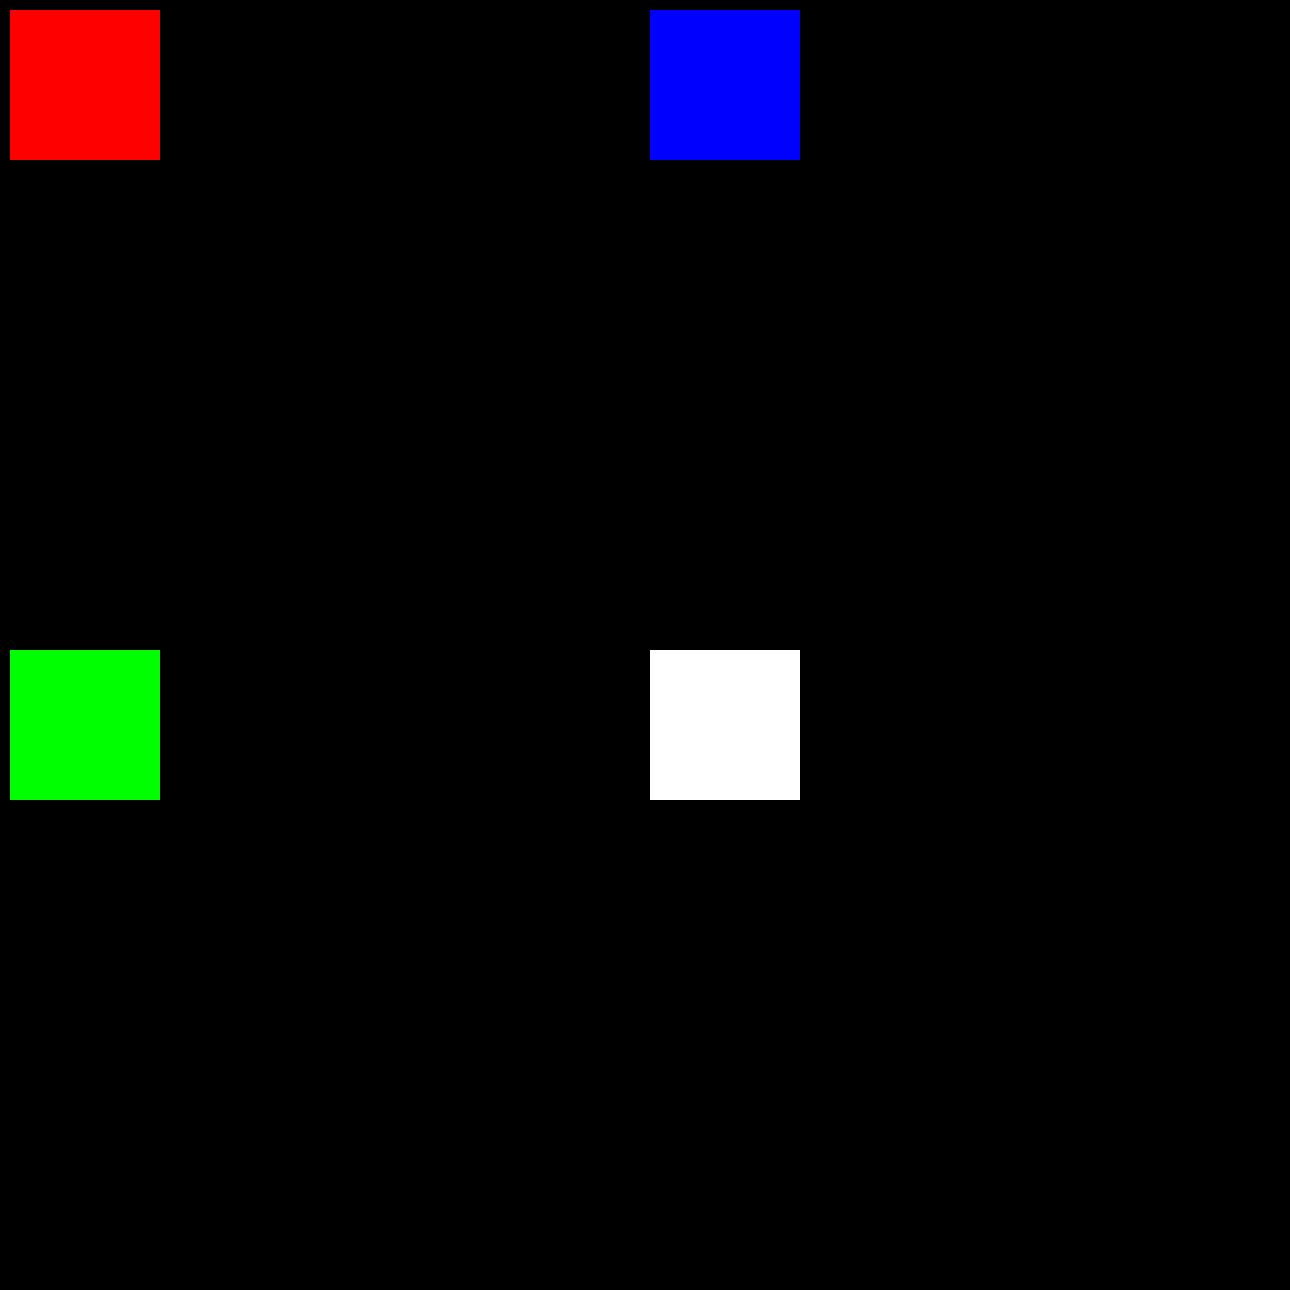
\includegraphics[width=0.28\textwidth]{2x2_1.png} 
\begin{center}
\vspace{-0.5em}
  Abb 2.
\vspace{0.5em}
\end{center}
\justify

Im ersten Schritt werden die einzelnen Pixel des ursprünglichen Bildes in ein temporäres Array gelegt und der Skalierung entsprechend im Speicher abgelegt. BMP-Dateien sehen vor, dass ein gewisses Alignment bzw. Padding beachtet wird. Im Fall von BMP-24 Dateien, muss jede Zeile des Bildes so ausgerichtet sein, dass die jeweiligen Speicheradresse ein Vielfaches von 4 Byte haben. Wenn die Breite des Bildes nicht durch 4 teilbar ist, muss ein Padding durchgeführt werden, indem zusätzliche Null-Bytes hinzugefügt werden, bis dieses 4 Byte-Alignment erreicht ist. Dieses Konzept zieht sich durch die komplette Implementierung und wird im Weiteren nur noch gelegentlich erwähnt.\\

\pagebreak

\centering
\includegraphics[width=0.28\textwidth]{"2x2_2"}
\begin{center}
\vspace{-0.5em}
  Abb 3.
\vspace{-0.5em}
\end{center}
\justify
Anschliessend werden alle eindeutigen Nachbarn der im Speicher liegenden Pixel gefärbt. Dies geschieht mit Hilfe einer Variable {\textit{radius.}} 
\begin{lstlisting}
int radius = (scaling - 1) / 2;
\end{lstlisting}
Die For-Schleife läuft für jede Reihe immer von -radius bis radius und wird jedes mal um 1 inkrementiert.
Für jeden Ursprungspixel wird somit Reihe für Reihe abgearbeitet und im Speicher die richtige Farbe gesetzt. Der Radius ist so definiert, dass keine fremden Pixel gefärbt werden können. 

\centering
\includegraphics[width=0.28\textwidth]{"2x2_3"}
\begin{center}
\vspace{-0.5em}
  Abb 4.
\vspace{-0.5em}  
\end{center}
\justify
Im nächsten Schritt wird der rechte Rand von den am nächstliegenden Pixel durchgängig gefärbt. Wie auch schon zuvor, wird hier die Funktion 
\begin{lstlisting}
memcpy(dest_ptr, src_ptr, n);
\end{lstlisting}
verwendet, um $n$ Bytes von {\textit{src}} nach {\textit{dest}} im Speicher zu kopieren. 
\begin{lstlisting}
if (scale_factor % 2 == 0) { //scaling ist gerade
    index = 1;
} else { //scaling ist ungerade
    index = 0;
}
\end{lstlisting}
Die Grösse von $n$ berechnet sich durch $n = 3 \times (radius + index)$. Somit wird immer eine weitere Reihe des Randes für jeden Schleifen-Durchlauf gefärbt.\\
Bei geradem Skalierfaktor entstehen Lücken, wie in der Einführung des Pixelwiederholungsverfahrens zu sehen ist. Diese müssen nach dem zuvor erklärten Schema geschlossen werden. Das heisst, vertikale Lücken erhalten die Farbe von linksliegenden Pixeln und horizontale Lücken werden in der Farbe von darüberliegenden Pixeln gefärbt. Diese Schritte umfassen Abb. 5 und Abb. 6. Bei ungeradem Skalierfaktor wird sofort zum letzten Schritt (Abb. 7) gesprungen. Dies liegt daran, dass sich zwei ursprüngliche Nachbarn die Pixelreihen immer eindeutig aufteilen können.\\\\

\centering
\includegraphics[width=0.28\textwidth]{"2x2_4"}
\begin{center}
\vspace{-0.5em}
  Abb 5.
\vspace{0.5em}  
\end{center}
\justify

Im folgenden Fall beträgt die Skalierung den Faktor 4, d.h. die Lücken müssen geschlossen werden. Zuerst werden die vertikalen Lücken abgearbeitet. \\

\begin{lstlisting}
for (size_t t = 0; t < length; t++) {
    temp = pixelAddresses[t];
    for (int i = -1 * radius; i <= radius; i++) {
        if (!(t < width && i > 0)) // überprüfen, ob out of bounds
            memcpy(result + temp + (radius + 1) * 3 + zoomedWidth * i,
                   result + temp,
                   sizeof(uint8_t) * 3);
    }
}
\end{lstlisting}
\vspace{1em} 
In der äusseren for-Schleife wird über alle ursprünglichen Pixel iteriert. In der inneren for-Schleife wird innerhalb einer Lückenreihe über jeden Pixel iteriert. Jedem einzelnen Pixel werden dann exakt 3 Byte übergeben, die sich bekanntermassen aus jeweils einem Byte an roten, blauen und grünen Farbwerten zusammensetzen. \\

\pagebreak

\centering
\includegraphics[width=0.27\textwidth]{"2x2_5"}
\begin{center}
\vspace{-0.5em}
  Abb 6.
\vspace{-0.5em}  
\end{center}
\justify

Im vorletzten Schritt wird ersichtlich, wieso es sinnvoll war, den rechten Pixelrand bereits korrekt auszufüllen. Da es nun keine vertikalen Lücken mehr zwischen zwei ursprünglichen Nachbarn gibt, werden die horizontalen Lücken mit Leichtigkeit geschlossen.
\begin{lstlisting}
for (size_t t = 0; t < length; t += width) {
    temp = pixelAddresses[t];
    memcpy(result + temp - zoomedWidth * (radius + 1),
           result + temp,
           sizeof(uint8_t) * 3 * width * scale_factor);
}
\end{lstlisting}
Der Vorteil an dieser Implementierung ist, dass eine ganze horizontale Reihe aufeinmal dupliziert werden kann, indem $(witdh \times scale \times 3)$ Byte von der Zeile darüber in die gesamte horizontale Lücke geschrieben werden.\\

\centering
\includegraphics[width=0.27\textwidth]{"2x2_6"}
\begin{center}
\vspace{-0.5em}
  Abb 7.
\vspace{-0.5em}  
\end{center}
\justify
Im letzten Schritt wird nun der untere Rand durchgängig befüllt mit den darüberliegenden Pixeln. Auch hier wird in jedem Schleifen-Durchlauf immer eine ganze Zeile auf einmal dupliziert, sodass in diesem Beispiel die Schleife nur einmal laufen muss.
Eine mögliche Optimierung könnte die Verwendung von SIMD-Vektorisierung sein, um die direkten Nachbarn der Pixel schneller abzuarbeiten. Das potenzielle Problem besteht jedoch darin, dass die Quell- und Zieladressen für diese memcpy-Aufrufe über die Iterationen hinweg nicht konstant sind. In jeder Iteration werden die Adressen auf der Grundlage der aktuellen Indizes und verschiedener anderer Parameter berechnet. SIMD-Instruktionen sind am effizientesten, wenn die Daten, auf die sie angewendet werden, in einem regelmäßigen, vorhersagbaren Muster im Speicher angeordnet sind, was hier unter anderem wegen dem Padding nicht der Fall ist.

\pagebreak

\section{Korrektheit/Genauigkeit}
{\textbf{Korrektheit der Implementierung von window()}}
\newline Um die Korrektheit der Implementierung zu überprüfen, wurden einige repräsentative Unit-Tests entwickelt.\newline
\textbf{Testfall für ein Fenster der Grösse 1x1:}\hspace{0.5cm} Es wird ein kleines Bild mit einem einzelnen Pixel erstellt, und die Funktion window wird aufgerufen, um ein Fenster der Grösse 1x1 zu erstellen. Das erwartete Ergebnis ist das Pixel selbst.
\newline \emph{Beispielhafter Auszug des Tests:}
\begin{lstlisting}
void test_window_single_pixel() {
    uint8_t img[3] = { 255, 0, 0 }; // Ein roter Pixel
    uint8_t result[3];
    window(img, 0, 0, 1, 1, result, 1, 1);
    // Erwartetes Ergebnis: Der rote Pixel
    assert(result[0] == 255 && result[1] == 0 && result[2] == 0);
}
\end{lstlisting}
\textbf{Testfall für ein Fenster der Grösse 2x2:}\hspace{0.5cm} Ein Bild mit 4 Pixeln wird erzeugt, und die Funktion window wird aufgerufen, um ein Fenster der Grösse 2x2 zu erstellen. Das erwartete Ergebnis ist das ausgewählte Fenster mit den entsprechenden Pixeln.\newline 
\textbf{Testfall für ein Fenster ausserhalb des Bildes:}\hspace{0.5cm} Es wird ein Bild mit einer Breite von 3 Pixeln und einer Höhe von 2 Pixeln erstellt. Die Funktion window wird aufgerufen, um ein Fenster der Grösse 2x2 mit den Koordinaten (2, 1) zu erstellen. Das erwartete Ergebnis ist ein leeres Fenster, da sich das Fenster ausserhalb des Bildes befindet.\newline 
\textbf{Testfall für ein grösseres Fenster:}\hspace{0.5cm} Es wird ein Bild mit einer Breite von 4 Pixeln und einer Höhe von 3 Pixeln erstellt. Die Funktion window wird aufgerufen, um ein Fenster der Grösse 3x2 mit den Koordinaten (1, 1) zu erstellen. Das erwartete Ergebnis ist das ausgewählte Fenster mit den entsprechenden Pixeln.\newline 
{\textbf{Korrektheit der Implementierung von zoom():}}\hspace{0.5cm}
Die Implementierung stellt sicher, dass die skalierten Pixel korrekt verändert werden und die Tie-Breaker-Regel ordnungsgemäss angewendet wird, um Nachbarpixel zu kopieren. Dies gewährleistet, dass die skalierten Bilder die richtigen Informationen enthalten und eine genaue Repräsentation des Originalbildes darstellen. Die Korrektheit des Skalierungsalgorithmus wird durch automatisierte Tests überprüft, die repräsentative Beispiele für verschiedene Skalierungsfaktoren und Bildgrössen enthalten. \\\\
\textbf{Unit Tests (Beschreibung):} \\\\
\textbf{Testfall: Skalierungsfaktor 1}\hspace{0.5cm}
Überprüft, ob das skalierte Bild mit einem Skalierungsfaktor von 1 identisch zum Originalbild ist.
\textbf{Testfall: Skalierungsfaktor grösser als 1:}\hspace{0.5cm}
Überprüft, ob das skalierte Bild die richtige Anzahl von Pixeln basierend auf dem Skalierungsfaktor enthält.
\newline \textbf{Testfall: Randfälle:}\hspace{0.5cm}
Überprüft die korrekte Behandlung von Randpixeln und -bereichen beim Skalieren.
\pagebreak

\emph{Beispielhafter Auszug der Tests:}
\begin{lstlisting}
void test_zoom_scale_factor_3() {
    // Arrange
    uint8_t img[24] = {255, 0, 0,    // Rot
                       0, 0, 255,    // Blau
                       0, 255, 0,    // Grün
                       255, 255, 255}; // Weiss
    size_t width = 2;
    size_t height = 2;
    size_t scale_factor = 3;
    uint8_t result[72]; // Skaliertes Bild mit 6x6 Pixeln (24 Bytes pro Pixel)
    zoom(img, width, height, scale_factor, result, 0);
    // Assert
    assert(result[0] == 255);    // Rot
    assert(result[1] == 0);
    assert(result[2] == 0);
    assert(result[3] == 255);    // Rot
    assert(result[4] == 0);
    assert(result[5] == 0);
    // ...
    // result[18] = padding
    // result[19] = padding
    // ...
    assert(result[69] == 255);   // Weiss
    assert(result[70] == 255);
    assert(result[71] == 255);
}
\end{lstlisting}
\section{Performanzanalyse}

Nach einigen Tests auf dem Server der lxhalle mit verschiedenen Skalierungsfaktoren und Fenstergrößen konnten wir folgende Ergebnisse in einer Tabelle zusammenstellen.

\begin{table}[h]
\centering
\begin{tabular}{|c|c|c|c|c|}
\hline
\textbf{Fenstergröße} & \textbf{Skalierungsfaktor} & \textbf{Durchschnittliche Ausführungszeit (Sek.)}\\
\hline
128x128     & 1            & 0.014315 \\
128x128     & 2            & 0.022671 \\
128x128     & 4            & 0.036589 \\
128x128     & 8            & 0.072948 \\
\hline
512x512     & 1            & 0.060576 \\
512x512     & 2            & 0.090332 \\
512x512     & 4            & 0.202651 \\
512x512     & 8            & 0.618855 \\
\hline
1024x1024   & 1            & 0.163903 \\
1024x1024   & 2            & 0.274887 \\
1024x1024   & 4            & 0.758264 \\
1024x1024   & 8            & 4.273953 \\
\hline
2048x2048   & 1            & 0.339196 \\
2048x2048   & 2            & 0.832601 \\
2048x2048   & 4            & 3.018189 \\
2048x2048   & 8            & 9.704604 \\
\hline
\end{tabular}
\end{table}

Aus der Tabelle geht hervor, dass sich die Ausführungszeit etwa verdoppelt, wenn der Skalierungsfaktor verdoppelt wird (bei konstanter Fenstergröße). Dies deutet darauf hin, dass der Skalierungsfaktor zu einer linearen ($O(n)$) Zeitkomplexität beiträgt.

Ähnlich verhält es sich, wenn wir die Veränderung der Ausführungszeit betrachten, während die Fenstergröße vervierfacht wird (bei konstantem Skalierungsfaktor). Wir sehen, dass sich die Zeit ebenfalls etwa vervierfacht. Da wir mit zwei Dimensionen (Höhe und Breite) arbeiten, deutet eine Vervierfachung der Gesamtgröße bei einer Vervierfachung der Zeit darauf hin, dass die Fenstergröße ebenfalls zu einer linearen ($O(n)$) Zeitkomplexität beiträgt.

Zusammenfassend lässt sich beobachten, dass sowohl die Fenstergröße als auch der Skalierungsfaktor linear zur Zeitkomplexität beiträgt. 


\section{Zusammenfassung und Ausblick}

In dieser Arbeit wurde ein kleiner Einblick in die digitale Bildverarbeitung gegeben anhand von Pixelmanipulation. Es wurde sich stets auf Bilder des Formats BMP-24 konzentriert und dieses näher beschrieben. Für die Pixelmanipulation wird zunächst ein Teilbereich eines Bildes ausgewählt und dieser im Anschluss nach dem Pixelwiederholungsverfahren vergrößert. Zunächst wurden die direkten Nachbarn von den ursprünglichen Pixeln gefärbt und im Anschluss die Lücken nach einem gewählten Prinzip geschlossen, sodass am Ende alle Pixel passend gefärbt sind. 
Es bleibt festzuhalten, dass Bilder mit dem BMP-24-Format besonders geeignet sind für qualitativ hochwertige Bilder, auf der anderen Seite ist aber der daraus resultierende hohe Speicherverbrauch nicht zu vernachlässigen. In einem kurzen Ausblick kann genannt werden, dass es in der Tat sinnvoll gewesen wäre, die direkten Nachbarn mit der vektorisierten SIMD-Implementierung zu färben, es aber große Herausforderungen darstellt die Speicherverwaltung so zu gestalten, dass SIMD-Vektorisierung kein Risiko darstellt. 

% TODO: Fuegen Sie Ihre Quellen der Datei Ausarbeitung.bib hinzu
% Referenzieren Sie diese dann mit \cite{}.
% Beispiel: CR2 ist ein Register der x86-Architektur~\cite{intel2017man}.
\bibliographystyle{plain}
\bibliography{Ausarbeitung}{}


\end{document}